\documentclass[11pt]{article}

\usepackage[margin=1.1in]{geometry}
\usepackage[T1]{fontenc}
\usepackage[utf8]{inputenc}
\usepackage{lmodern}
\usepackage{microtype}
\usepackage{amsmath,amssymb}
\usepackage{booktabs}
\usepackage{graphicx}
\usepackage{xcolor}
\usepackage{listings}
\usepackage[numbers,sort&compress]{natbib}
\usepackage[hidelinks]{hyperref}

\graphicspath{{figures/}}

\lstset{
  basicstyle=\ttfamily\small,
  breaklines=true,
  columns=fullflexible,
  frame=single,
  framerule=0.2pt,
  xleftmargin=1em,
  keepspaces=true,
}

\newcommand{\pytracer}{\textsc{Pytracer}}
\newcommand{\pyt}{\textsc{Pytracer~2}}
\newcommand{\pytone}{\textsc{Pytracer~1}}
\newcommand{\sig}{\operatorname{sig}}

\title{Pytracer 2: Honest Tiered Instrumentation for\\
Numerical Variability Profiling in Python}

\author{%
  Yohan Chatelain\\
  \small\texttt{yohan.chatelain@gmail.com}%
}

\date{Draft of \today}

\begin{document}

\maketitle

\begin{abstract}
% abstract — filled in during prose pass
TODO abstract

\end{abstract}

% intro — filled in during prose pass
\section{Introduction}

% background — filled in during prose pass
\section{Background}

\section{Design}
\label{sec:design}

Figure~\ref{fig:architecture} shows the pipeline: instrumentation tiers
emit a schema-versioned event stream; events are captured append-only and
finalized to columnar storage; runs are aligned call-by-call; aggregation
attributes digit loss to functions; and the results feed reports, an
interactive dashboard, and CI gates.

\begin{figure}[t]
  \centering
  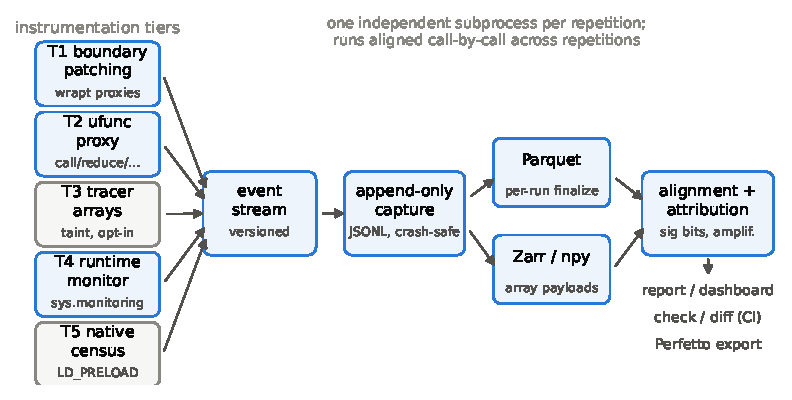
\includegraphics[width=\linewidth]{architecture}
  \caption{\pyt{} architecture. Five instrumentation tiers (left) feed a
  schema-versioned event stream captured append-only (crash-safe JSONL),
  finalized per run to Parquet with array payloads in Zarr. Runs are
  aligned call-by-call and aggregated into digit-loss attribution,
  consumed by reports, the dashboard, CI gates, and a Perfetto export.}
  \label{fig:architecture}
\end{figure}

\subsection{The instrumentation problem, stated honestly}
\label{sec:design-problem}

The central tension of dynamic numerical tracing is
\emph{transparency} (observe every numerical operation without the user
changing code) versus \emph{specificity} (each interception mechanism
works only for particular kinds of callables, and the aggressive
mechanisms alter the semantics of the traced program). PyTracer\,1
resolved the tension in favor of transparency by patching
\texttt{builtins.type} and \texttt{isinstance} process-wide so that
wrapped objects would masquerade as their originals --- the cautionary
tale that motivates this design: a tracer must not change the meaning of
the program it observes.

\pyt{} instead composes five tiers, each a separate module with a
declared contract (Table~\ref{tab:tiers}). The default configuration
(\texttt{hybrid} = T1+T2+T4) is safe: it never proxies a returned value,
never alters a type observable by user code, and its blind spots are
enumerated by the deeper tiers and the coverage report.

\begin{table}[t]
  \centering\small
  \caption{The tier contract. ``Sees'' and ``blind to'' are declared in
  documentation and enforced by the conformance test suite; overheads are
  measured in Section~\ref{sec:eval-overhead}.}
  \label{tab:tiers}
  \begin{tabular}{@{}lp{3.4cm}p{3.2cm}lll@{}}
    \toprule
    Tier & Sees & Blind to & Overhead & Risk & Default \\
    \midrule
    T1 patch & targeted Python functions/methods & aliases, operators,
      C-internal & low & low & on \\
    T2 ufunc & targeted ufuncs incl.\ \texttt{reduce},
      \texttt{accumulate}, \texttt{out=} & operator dispatch, C-internal
      & low--med & low & on \\
    T3 tracer array & all NumPy ops on tainted data, alias-proof & taint
      stripped at \texttt{asarray}/C entry & high & med & off \\
    T4 monitor & call graph, C-call occurrence, line coverage & operand
      values & med & low & on \\
    T5 native census & BLAS/LAPACK kernels + shapes, incl.\ from Cython &
      operand values, non-BLAS C & low & low--med & off \\
    \bottomrule
  \end{tabular}
\end{table}

\textbf{T1 --- boundary patching} wraps targeted Python-level functions
and methods (plugin lists plus user \texttt{--target} globs) using
\texttt{wrapt} proxies~\citep{wrapt}, which transparently forward
\texttt{\_\_name\_\_}, signatures, and \texttt{isinstance} via
\texttt{\_\_class\_\_}. The wrapped call emits input events, calls the
original, emits output events, and returns the result object
\emph{unchanged} --- never copied, never proxied.

\textbf{T2 --- ufunc interception} answers the ufunc specificity problem
with a dedicated \texttt{UfuncProxy}: it intercepts \texttt{\_\_call\_\_},
\texttt{reduce}, \texttt{reduceat}, \texttt{accumulate}, \texttt{outer},
and \texttt{at} --- each tagged with the method name, since a
\texttt{reduce} is numerically a different operation than an elementwise
call --- handles \texttt{out=} buffers (summarized after the call,
flagged in-place), and keeps \texttt{isinstance(numpy.add, np.ufunc)}
true. Its declared blind spot is operator dispatch, covered by T3.

\textbf{T3 --- tracer arrays} (opt-in, \texttt{--instrument taint}) close
the operator gap for selected data: values tagged with
\texttt{pytracer.taint(x)}, plus outputs of traced calls, become
\texttt{TracedArray} instances whose \texttt{\_\_array\_ufunc\_\_} and
\texttt{\_\_array\_function\_\_} protocols observe \emph{every} NumPy
operation on them --- including \texttt{a + b} and \texttt{a @ b} and
calls made from third-party Python code --- regardless of aliasing,
because protocol dispatch keys on the operand type, not on how the
function was looked up. Taint is stripped by \texttt{np.asarray} at many
C entry points, so T1 wrappers re-taint their outputs to re-seed
propagation. T3 alters \texttt{type(x)} checks and is therefore never a
default: it is the drill-down instrument for a region T1/T2 already
localized.

\textbf{T4 --- runtime monitor} uses \texttt{sys.monitoring}
(PEP\,669~\citep{pep669}; hence the Python $\geq$ 3.12 floor) to record
structure only: the call graph that gives every event its parent call,
per-line execution counts whose cross-run differences localize
control-flow divergence, and --- centrally for coverage honesty --- a
census of calls to C callables that had \emph{no} wrapper installed. The
monitor cannot see operand values, but it can prove that
\texttt{numpy.mean} ran 2{,}000 times unobserved, which is exactly what
the coverage report and the \texttt{suggest-targets} workflow need.

\textbf{T5 --- native kernel census} (opt-in, \texttt{--native}, Linux)
is a small \texttt{LD\_PRELOAD} shim interposing BLAS/LAPACK dynamic
symbols (\texttt{dgemm\_}, \texttt{dgesv\_}, \ldots, including the
prefixed ILP64 symbols shipped in NumPy/SciPy wheels). It records which
kernels ran and their dimensions --- including calls from Cython that
never touch a Python object --- but not operand values: it is a coverage
and attribution instrument, not a value tracer. Value-level perturbation
of these kernels is the perturbation engine's job.

\subsection{Execution model}
\label{sec:design-exec}

Each repetition is an independent subprocess: in-process repeats would
share module caches, RNG state, and perturbation-backend seeds, and one
crash would kill the experiment. The child installs instrumentation
\emph{before} importing the target script, executes it as
\texttt{\_\_main\_\_}, and finalizes its trace in a \texttt{finally}
block. Per-run environment overrides from the \texttt{[perturb.env]}
config table (with \texttt{\{run\_index\}} substitution) rotate MCA seeds
for engines like Verificarlo. Run metadata captures an
\emph{allowlisted} subset of the environment only (\texttt{PATH},
\texttt{OMP\_*}, \texttt{VFC\_*}, \ldots) --- never the raw environment,
so secrets cannot leak into shareable trace directories.

\subsection{Events, storage, and crash-safety}
\label{sec:design-storage}

Every event is a schema-versioned \texttt{msgspec} struct: run, call and
parent-call identifiers, tier, callsite, per-callsite occurrence counter,
phase (input/output/exception), and a numeric summary (dtype, shape,
moments, norms, NaN/Inf/subnormal counts, and a fingerprint). During
capture, events are appended as JSON lines --- a crash loses at most the
final partial line. At run finalization the capture is converted to
\texttt{events.parquet} for analysis and interoperability
(pandas/duckdb); array payloads go to Zarr with zstd compression under
the \texttt{store\_arrays} policy. Parquet is deliberately \emph{not}
written during capture: row-group buffering plus a crash yields truncated
files, whereas the JSONL capture of a SIGKILLed run remains readable
(measured in Section~\ref{sec:eval-storage}). No pickle format appears
anywhere in the system.

\subsection{Alignment}
\label{sec:design-alignment}

Cross-run metrics require knowing which call in run 3 corresponds to
which call in run 7. The unit of alignment is the \emph{call} (aligning
input and output events independently mismatches them when counts
diverge), keyed by module, qualified name, callsite, ufunc method, and a
deterministic per-callsite occurrence counter. Three modes:
\texttt{strict} requires identical call sequences and fails loudly at the
first divergence (doubling as the determinism test); \texttt{callsite}
(default) matches by callsite key and occurrence index;
\texttt{fuzzy} performs per-callsite longest-common-subsequence matching
using input shapes and dtypes as hints, so unmatched calls become
missing/extra records instead of cascading misalignment. The alignment
report also carries the T4 line-count divergence table, which localizes
control-flow divergence even inside untraced code.

\subsection{Metrics: digit-loss attribution}
\label{sec:design-metrics}

For every aligned call group, \pyt{} computes significant bits of each
input and output across runs, on one of two bases, never conflated:
\emph{element} --- true element-wise significant digits computed from
stored array payloads (the real measurement); or \emph{summary} ---
$\sig(\mathrm{mean})$, the cross-run stability of the argument's mean,
used when payloads were not stored and labeled as the optimistic proxy it
is. Every derived metric row carries its \texttt{sig\_basis}.

The headline metric is per-call \emph{amplification}:
\begin{equation}
  \mathrm{amp} \;=\; \sig_{\min}(\text{inputs}) \;-\;
  \sig_{\min}(\text{outputs}),
  \label{eq:amp}
\end{equation}
the bits of precision destroyed by the call itself. Ranking functions by
amplification first, absolute output significance second, and
control-flow divergence third separates the \emph{sources} of instability
from its \emph{victims} --- the question users actually have. NaN/Inf
instability (an output that is NaN in some runs but not others) is
flagged independently.

\subsection{Coverage accounting and the discovery loop}
\label{sec:design-coverage}

Coverage analysis merges (a) events observed per tier, (b) the T4 census
of C callables invoked with no wrapper --- which doubles as the
\texttt{suggest-targets} list --- and (c) T5 native kernels with no
correlated traced call. The report renders this as an
observed/unobserved section with two structural notes that are always
present: operator dispatch on ndarrays is not observable at T1/T2, and
calls inside compiled extensions are invisible to every Python tier. The
discovery loop is then: run cheaply with the monitor, let
\texttt{suggest-targets} propose wrappers for what it saw, re-run with
those targets, and drill into localized regions with taint mode.

\subsection{Numerical CI}
\label{sec:design-ci}

\texttt{pytracer check} evaluates an experiment against thresholds
(minimum significant bits, maximum divergence, NaN/Inf policies; also read
from \texttt{pytracer-thresholds.toml}) and exits nonzero on violation,
making stability a regression-testable property. \texttt{pytracer diff}
compares two experiments function-by-function and, with
\texttt{--fail-on-regression}, gates on significance drops beyond a
tolerance --- the A/B instrument for library upgrades, precision changes,
and flag flips (exercised in Section~\ref{sec:eval-case}).

% implementation — filled in during prose pass
\section{Implementation}

% evaluation — filled in during prose pass
\section{Evaluation}

\section{Related Work}
\label{sec:related}

\paragraph{Perturbation engines.}
Verificarlo~\citep{denis2016verificarlo} instruments floating-point
operations at LLVM compile time with interchangeable backends (MCA,
cancellation detection); Verrou~\citep{fevotte2017verrou} achieves the
same dynamically under Valgrind without recompilation;
CADNA~\citep{jezequel2008cadna} implements CESTAC with synchronous
triplicated execution. Fuzzy system libraries randomize \texttt{libm}
itself, enabling container-level perturbation of unmodified pipelines,
an approach used to quantify condition-level uncertainty in neuroimaging
analyses~\citep{kiar2021comparing}. \pyt{} sits deliberately above all of
these: they make runs vary, it explains where the variation came from.
File-based localization~\citep{salari2020spot} attributes pipeline
variability at the granularity of intermediate files; \pyt{} works at the
granularity of function calls within one process.

\paragraph{Numerical debugging and repair.}
FpDebug~\citep{benz2012fpdebug} shadows every operation with
high-precision values under Valgrind;
Herbgrind~\citep{sanchezstern2018herbgrind} tracks error back to root
causes in binaries; Herbie~\citep{panchekha2015herbie} rewrites
floating-point expressions for accuracy, and
FPTaylor~\citep{solovyev2015rigorous} bounds round-off error of small
expressions rigorously; FPBench~\citep{damouche2017fpbench} standardizes
their benchmarks. These tools analyze expressions or compiled binaries;
none observes the Python/C boundary where scientific Python programs
actually spend their numerical effort, and none addresses the coverage
question --- what fraction of a NumPy/sklearn workload the analysis saw
--- that \pyt{} makes a first-class output.

\paragraph{Tracing numerical behavior in context.}
VeriTracer~\citep{chatelain2019veritracer} added temporal, contextualized
traces of significance to Verificarlo at the C/Fortran level.
PyTracer~\citep{chatelain2023pytracer} brought instability profiling to
Python via import hooks and is this work's direct predecessor;
Section~\ref{sec:eval-v1} quantifies its current state, and
Sections~\ref{sec:design}--\ref{sec:implementation} describe how \pyt{}
replaces its global \texttt{builtins} patching with tiered, contracted
instrumentation, its pickle trace format with schema-versioned columnar
storage, and its silent truncation with explicit alignment. The PEP\,669
monitoring API~\citep{pep669} that \pyt{} builds on was designed for
low-overhead tooling and, to our knowledge, \pyt{} is the first numerical
QA tool built on it. NumPy's array protocols
(\texttt{\_\_array\_ufunc\_\_}, \texttt{\_\_array\_function\_\_})
\citep{harris2020numpy} are the mechanism behind tier T3, used elsewhere
for units, autodiff, and lazy evaluation; \pyt{} repurposes them for
alias-proof observation.

% conclusion — filled in during prose pass
\section{Conclusion}


\bibliographystyle{plainnat}
\bibliography{refs}

\end{document}
